\documentclass[12pt]{article}

\usepackage{amsmath}
\usepackage{unicode-math}
\usepackage{xltxtra}
\usepackage{xgreek}

\setmainfont{Liberation Serif}

\usepackage{tabularx}

\pagestyle{empty}

\usepackage{geometry}
 \geometry{a4paper, total={190mm,280mm}, left=10mm, top=10mm}

 \usepackage{graphicx}
 \graphicspath{ {images/} }

 \usepackage{wrapfig}
\usepackage{lipsum}%% a garbage package you don't need except to create examples.

\begin{document}

\section*{Θέμα Α}
  \noindent
  \begin{enumerate}
    \item \textbf{[Μονάδες 15]} Απόδειξη από το βιβλίο.
    \item \textbf{[Μονάδες 10]} Σ, Σ, Λ, Λ, Σ
  \end{enumerate}

\section*{Θέμα Β}
  \noindent
  \begin{enumerate}
    \item \textbf{[Μονάδες 5]} Με Πυθαγόρειο $ΑΖ^2=ΑΔ^2-ΔΖ^2 \implies ΑΖ=4$
    \item \textbf{[Μονάδες 5]} Εμβαδό παραλληλογράμμου $ΔΕ\cdot ΑΖ=4 \cdot 4=16$
    \item \textbf{[Μονάδες 5]} Εμβαδό τραπεζίου $\frac{(Β+β)υ}{2}=28$
    \item \textbf{[Μονάδες 5]} $Ε=\frac{αβγ}{4R} \implies R=\frac{150}{48}$
    \item \textbf{[Μονάδες 5]} $Ε=τ\cdot ρ \implies ρ=\frac{12}{8}$
  \end{enumerate}

\section*{Θέμα Γ}
  \noindent
    \begin{enumerate}
    \item \textbf{[Μονάδες 9]} Μήκος ημικυκλίου, $l=3\frac{\pi R}{2}aR=\pi R$
    \item \textbf{[Μονάδες 4]} Με Πυθαγόρειο $υ^2=4R^2-R^2 \implies υ=R \sqrt{3}$
    \item \textbf{[Μονάδες 3]} Εμβαδό τριγώνου $\frac{β\cdot υ}{2}=R^2 \sqrt{3}$
    \item \textbf{[Μονάδες 9]} Εμβαδό τριγώνου εκτός ενός ημικυκλίου, $R^2 \sqrt{3} - \pi \frac{R^2}{2}$
  \end{enumerate}

\section*{Θέμα Δ}
  \noindent
  \begin{enumerate}
    \item \textbf{[Μονάδες 5]} Με γενικευμένο Πυθαγόρειο $ΑΓ^2=ΒΓ^2+ΑΒ^2-2ΑΒ\cdot ΒΓ \cdot συν\hat{Β} \implies ΑΓ=10$
    \item \textbf{[Μονάδες 5]} Με ανίσωση $ΒΓ^2>ΑΓ^2+ΑΒ^2$
    \item \textbf{[Μονάδες 5]} Με γενικευμένο Πυθαγόρειο $ΒΓ^2=ΑΓ^2+ΑΒ^2+2ΑΓ\cdot ΑΔ \implies ΑΔ=20$
    \item \textbf{[Μονάδες 5]} Με προβολή κάθετης στην υποτείνουσα $ΑΕ \cdot ΑΒ = ΑΔ^2 \implies ΑΕ=16$
    \item \textbf{[Μονάδες 5]} Απο πριν $ΒΕ=ΑΒ-ΒΕ=9$. Άρα με προβολές στην υποτείνουσα $ΔΕ^2=ΒΕ\cdot ΑΕ \implies ΔΕ=12$
  \end{enumerate}

  \begin{figure}[h]
    \centering
    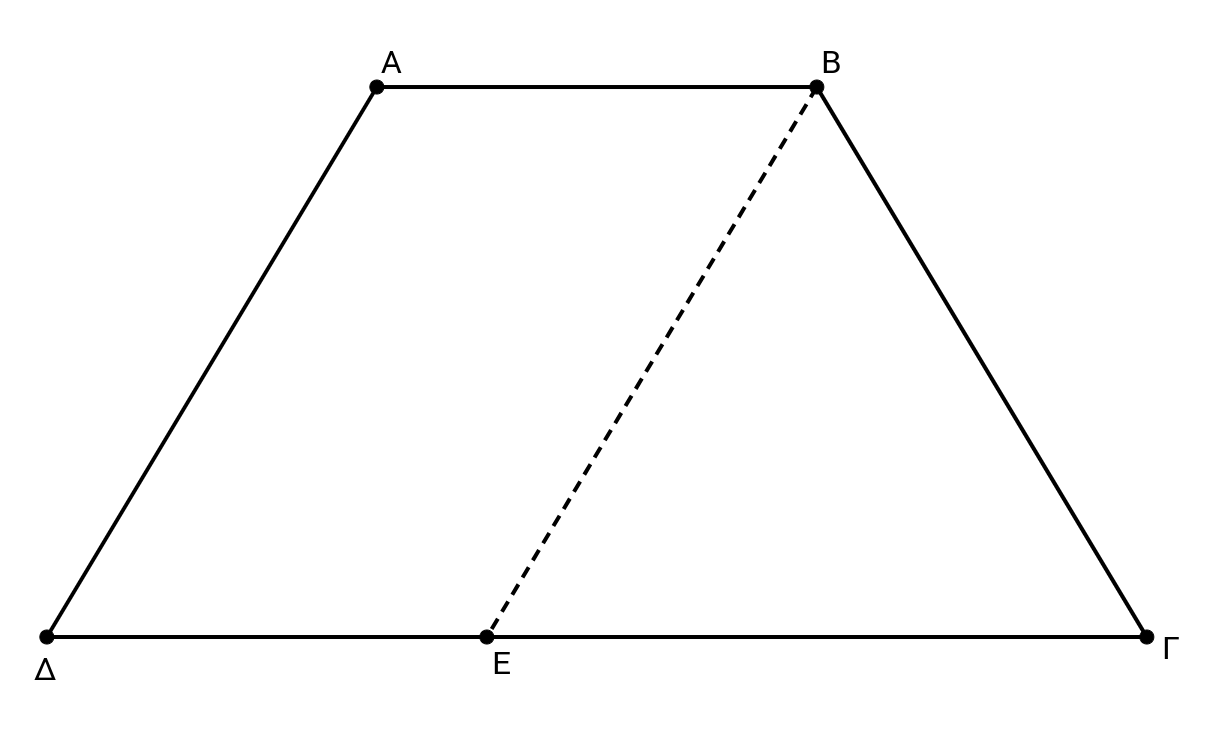
\includegraphics[scale=0.12]{2017BGeo2}
    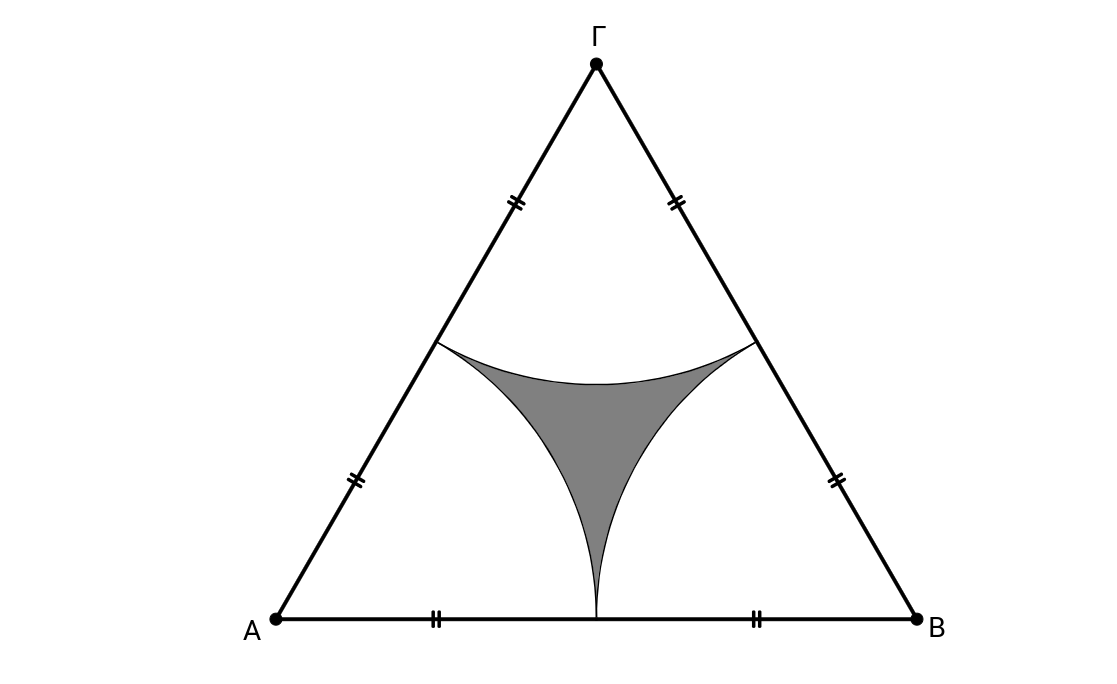
\includegraphics[scale=0.12]{2017BGeo3}
    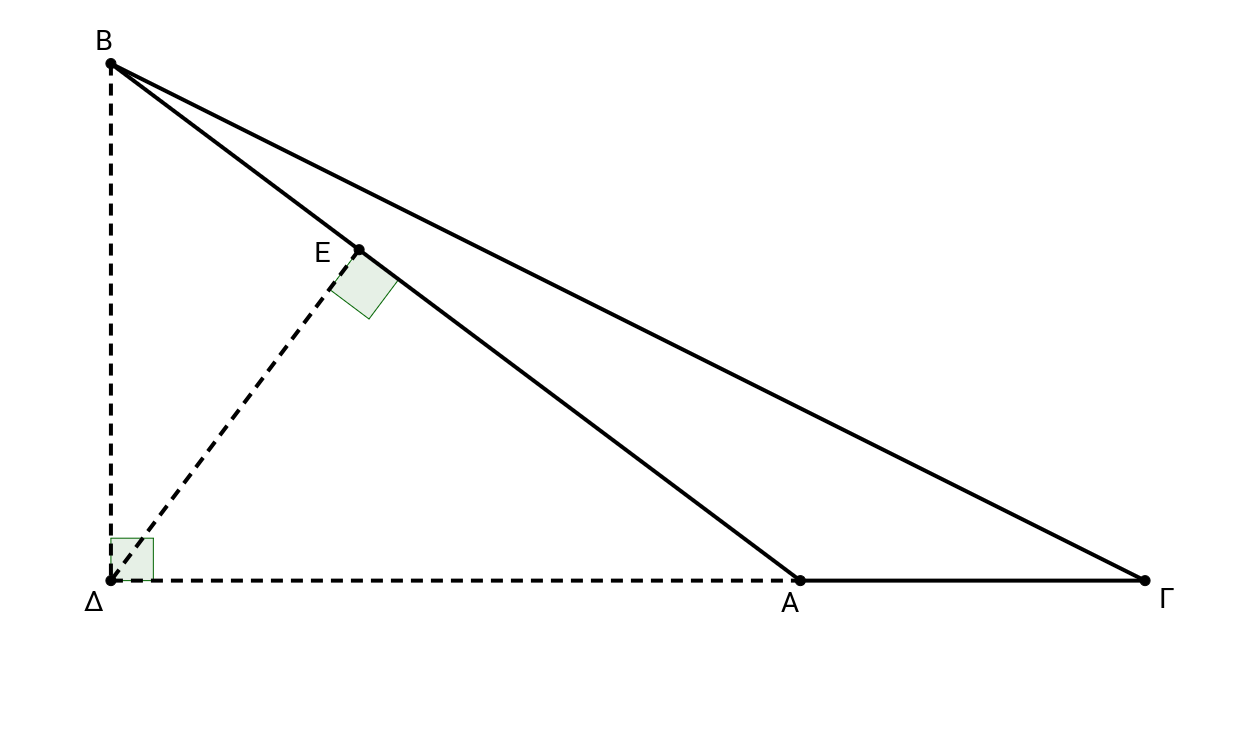
\includegraphics[scale=0.12]{2017BGeo4}
  \end{figure}
\end{document}
